\documentclass{article}
\usepackage{amsmath, amssymb, amssymb}
\usepackage{tikz}
\usepackage{tikz-3dplot}

\begin{document}
\begin{center}
    \begin{LARGE}
        \textbf{Calculus II}
    \end{LARGE}
\end{center}

\section{Vectors}

$\mathbb{R}$ represents the set of real numbers.\\[1pt]
$\mathbb{R}^2$ represents a 2 dimensional real plane. \\[1pt]
\[\mathbb{R}^2 = \{(x,y) \mid x,y \in \mathbb{R}\}\]

\begin{figure}[h]
\centering
\begin{tikzpicture}
    \draw[<->] [black, ultra thin] (-3,0) -- (3,0);
    \draw[<->] [black, ultra thin] (0,-2) -- (0,2);
    \filldraw[black] (0,0) circle (1pt) node[anchor=north west] {O};
    \draw[->][black, thick] (0,0) -- (1,1) node[anchor=south west] {$(1,1)$} node[anchor=south east] {$\vec{v}$};
    \draw[->][black, thick] (0,0) -- (1,0) node[anchor=south west] {$(1,0)$} node[anchor=north] {$\vec{u}$};
    \draw[->][black, thick] (1,1) -- (1,0);
    \filldraw[black] (1,0.75) circle (0.05pt) node[anchor=west] {$\vec{v} - \vec{u}$};
\end{tikzpicture}%\\[1pt]
\end{figure}
Normally elements of $\mathbb{R}$ are known as scalers.\\[1pt]

$\cdot$ add (or subtract) two vectors

$\cdot$ if $c \in \mathbb{R}$ and $v \in \mathbb{R}^2$,  $c\vec{v}$ 

\subsection{Dot Product}
$u = (u_1, u_2)$ and $v = (v_1, v_2)$ \[u.v = u_1.v_1 + u_2.v_2\]

\subsubsection*{Theorem}
\[u.v = |u||v| \cos(\theta)\]
where $\theta$ is the angle between $\vec{u}$ and $\vec{v}$
and $|u|$ is the length of vector $\vec{u}$

\begin{figure}[h]
    \centering
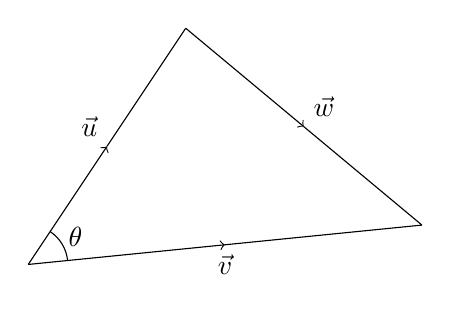
\begin{tikzpicture}
    \draw[->][black] (0,0) -- (1,1.5) node[anchor=south east] {$\vec{u}$};
    \draw [black] (1,1.5) -- (2,3);
    \draw[->] [black] (0,0) -- (2.5, 0.25) node[anchor=north] {$\vec{v}$};
    \draw [black] (2.5,  0.25) -- (5, 0.5);
    \draw[->] [black] (2,3) -- (3.5, 1.75) node[anchor=south west] {$\vec{w}$};
    \draw [black] (3.5, 1.75) -- (5, 0.5);
    \draw[black] (0.5, 0.05) arc (5.71:56.3:0.5);
    \draw[black] (0.6, 0.11) node[anchor=south] {$\theta$};
\end{tikzpicture}
\end{figure}
Proof:
\begin{align*}
    w^2 &= u^2 + v^2 - 2|u||v| \cos(\theta) \dots(1)\\
    \vec{w} &= \vec{v} - \vec{u}\\
    w &= (v_1 - u_1, v_2 - u_2)\\
    w^2 &= (v_1 - u_1)^2 + (v_2 - u_2)^2\\
    w^2 &= v_1^2 - 2v_1u_1 + u_1^2 + v_2^2 - 2v_2u_2 + u_2^2\\
    w^2 &= v^2 + u^2 - 2v_1u_1 - 2v_2u_2 \dots (2)\\
\end{align*}
now, as $(1) = (2)$

\begin{align*}
    u^2 + v^2 - 2|u||v| \cos(\theta) &= v^2 + u^2 - 2v_1u_1 - 2v_2u_2\\
    |u||v| \cos(\theta) &= v_1u_1 + v_2u_2\\
    |u||v| \cos(\theta) &= \vec{u}.\vec{v}\\
\end{align*}

Hence proved.\\[1pt]

Extending the above theorem to $\mathbb{R}^n$:
Consider $\vec{u} = (u_1, u_2, \dots, u_n), \vec{v} = (v_1, v_2, \dots, v_n) \in \mathbb{R}$
\[\vec{u}.\vec{v} = u_1v_1 + u_2v_2 + \dots + u_nv_n\]

\subsection{Unit Vectors}
If $\vec{v} \in \mathbb{R}^2$ is a vector.
then, \[\hat{v} = \frac{\vec{v}}{|\vec{v}|}\]

\subsection{Projections}
If $\vec{u}$ and $\vec{v}$ are vectors in $\mathbb{R}^2$ and $\theta$ is the angle between them:
\begin{figure}[h]
\centering
\begin{tikzpicture}
    \draw[black] (0,0) -- (2,1.5) node[anchor=south east] {$\vec{u}$};
    \draw[->] [black] (2,1.5) -- (4, 3);
    \draw[black] (0,0) -- (3, 0) node[anchor=north east] {$\vec{v}$};
    \draw[->] [black] (3,0) -- (6,0);
    \draw[black, loosely dashed] (4,3) -- (4,0);
    \draw[black] (3.8, 0) -- (3.8, 0.2);
    \draw[black] (4, 0.2) -- (3.8, 0.2);
\end{tikzpicture}
\end{figure}\\
let $\vec{w}$ be the projection of $\vec{u}$ on $\vec{v}$

\begin{align*}
    \vec{w} &= |u| \cos(\theta) \hat{v}\\
    \vec{w} &= \frac{|u| \cos(\theta)|v|\vec{v} }{|v|^2}\\
    \vec{w} &= \frac{\vec{u}.\vec{v}}{|\vec{v}|^2} \vec{v}\\
\end{align*}

\subsection{Cross Product}
Consider the vectors, $u,v$. Then the cross-product of $u$ and $v$ is defined as:
\[u \times v = |u||v|\sin(\theta) \hat{n}\]
where $\hat{n}$ is the unit vector perpendicular to the plane containing $u$ and $v$, and also $(\vec{u}, \vec{v}, \hat{n})$ form a right handed system.

\paragraph*{Properties of Cross Product: }
\begin{itemize}
    \item $\vec{u} \times \vec{v} = - (\vec{v} \times \vec{u})$
    \item $(r\vec{u}) \times (s \vec{v}) = rs \vec{u} \times \vec{v}$
    \item $ \vec{u} \times (\vec{v} + \vec{w}) = \vec{u} \times \vec{v} + \vec{u} \times \vec{w}$
\end{itemize}

$\vec{u}$ and $\vec{v}$ can also be represented as: 
\[ \vec{u} = u_1 \hat{i} + u_2 \hat{j} + u_3 \hat{k}\]
\[ \vec{v} = v_1 \hat{i} + v_2 \hat{j} + v_3 \hat{k}\]

\[\vec{u} \times \vec{v} = (u_2 v_3 - u_3 v_2)\hat{i} + (u_3 v_1 - u_1 v_3)\hat{i} + (u_1 v_2 - u_2 v_1)\hat{k}\]

\[\vec{u} \times \vec{v} = \begin{vmatrix}
    \hat{i} & \hat{j} & \hat{k} \\
    u_1 & u_2 & u_3\\
    v_1 & v_2 & v_3
\end{vmatrix}
\]
the above formula is only symbolic and meant to represent a cross product.

\section{Multi-Variable Calculus}

let $r: \mathbb{R} \rightarrow \mathbb{R}^3$ be a function.
(It could be to any $\mathbb{R}^n$)\\
for $t \in \mathbb{R}$, $r(t)$ is a vector in $\mathbb{R}^3$\\
\[r(t) = f(t)\hat{\imath} + g(t)\hat{\jmath} + h(t)\hat{k}\]

\subsection{Continuity}
$r$ is continuous at $a$ if: 
\[\lim_{t \rightarrow a} r(t) = r(a)\]
i.e. $\forall \epsilon > 0, \exists \delta > 0$ such that $|t - a| < \delta \implies |r(t) - r(a)| < \epsilon$

or, if $f$, $g$ and $h$ are continuous at $a$, $r$ is continuous at $a$.

\subsection{Differentiability}
%some random gibberish was taught
let $r: \mathbb{R} \rightarrow \mathbb{R}^3$ be a function. (We are taking $\mathbb{R}^3$ here, but it could be any $\mathbb{R}^n$)\\
the derivative of $r$ at $a$ is defined as:
\[ r'(a) = \lim_{t \rightarrow a} \frac{r(t) - r(a)}{t - a}\]
if 
\[r(t) = f(t)\hat{i} + g(t)\hat{j} + h(t)\hat{k}\]
\[r'(t) = f'(t)\hat{i} + g'(t)\hat{j} + h'(t)\hat{k}\]


\subsection{Integration}
let $f: [a,b] \rightarrow \mathbb{R}$ be a function.\\

the integral of $f$ from $a$ to $b$ is defined as:
\[\int_a^b f(x) dx = \text{Area under the curve $y = f(x)$ from $x = a$ to $x = b$}\]

\paragraph{Anti-derivative}let $f: [a,b] \rightarrow \mathbb{R}$ be a function.\\
\[ \int f(t) dt = F(t) +c \]
such that $F'(t) = f(t)$ and $c$ is an arbitrary constant

\paragraph{Fundamental Theorem of Calculus} let $f: [a,b] \rightarrow \mathbb{R}$ be a function and $F$ be its anti-derivative.\\
\[ \int_{a}^{b} f(t) dt = F(b) - F(a) \]

\subsubsection{Extending to a Vector Valued Function}
Consider a function $r: \mathbb{R} \rightarrow \mathbb{R}^3$ (we are taking $\mathbb{R}^3$ as an example, it could be any $\mathbb{R}^n$)\\
\[ r(t) = f(t)\hat{i} + g(t)\hat{j} + h(t)\hat{k} \]
\[\int_{a}^{b}r(t)dt = \int_{a}^{b}f(t)dt\hat{i} + \int_{a}^{b}g(t)dt\hat{j} + \int_{a}^{b}h(t)dt\hat{k} \]

\paragraph{Anti-derivative}
\[ \int r(t) dt = \left(\int f(t)dt + c_1\right)\hat{i} + \left(\int g(t)dt + c_2\right)\hat{j} + \left(\int h(t)dt + c_3\right)\hat{k}  \]
\[ \int r(t) dt = R(t) + C \]
where $R'(t) = r(t)$ and $C$ is an arbitrary constant vector.
\[ R(t) = F(t)\hat{i} + G(t)\hat{j} + H(t)\hat{k} \]
where $F'(t) = f(t)$, $G'(t) = g(t)$ and $H'(t) = h(t)$

\subsubsection{Length of a Curve}
let $r: [a,b] \rightarrow \mathbb{R}^3$ be a function. (As usual, we are taking $\mathbb{R}^3$, but it can be any $\mathbb{R}^n$)\\
the length of the curve $l$ from $a$ to $b$ is defined as:
\[ l = \int_{a}^{b} |r'(t)| dt \] 

\section{Multi-Variable Functions}
let $f: D \rightarrow \mathbb{R}$ be a function. Let $D\subseteq \mathbb{R}^n$. Then $f$ is called a Multi Variable Function\\
Eg: \[f(x,y) = \frac{1}{x^2 + y^2}\]
Domain of $f$ is $\mathbb{R}^2 - \{(0,0)\}$

\subsection{Limits}
let $f: D \rightarrow \mathbb{R}$ be a function. and $D\subseteq \mathbb{R}^2$. (we are taking $\mathbb{R}^2$ but it can be extended to any $\mathbb{R}^n$)\\

\[ \lim_{(x,y)\rightarrow (x_1, y_1)} f(x,y) = L\]

if $\forall \epsilon > 0, \exists \delta > 0$ such that $|(x,y) - (x_1, y_1)| < \delta \implies |f(x,y) - L| < \epsilon$
\\
Eg: \[ \lim_{(x,y)\rightarrow (0,0)} \frac{x^2 - xy}{\sqrt{x} - \sqrt{y}}\]
\[ \lim_{(x,y)\rightarrow (0,0)} \frac{x(x-y)}{\sqrt{x} - \sqrt{y}}\]
\[ \lim_{(x,y)\rightarrow (0,0)} x(\sqrt{x} + \sqrt{y})\]
\[ \therefore \lim_{(x,y)\rightarrow (0,0)} \frac{x^2 - xy}{\sqrt{x} - \sqrt{y}} = 0 \]
\\
Eg: \[ \lim_{(x,y)\rightarrow (0,0)} \frac{2x^2y}{x^4 + y^2}\]
this limit does not exist.\\

\subsection{Derivatives}
The usual definition of derivatives can't be extended to multi-variable functions.\\
Eg: \[ f(x,y) = x \]
\[ f'(x) = \lim_{(x,y)\rightarrow (x_1, y_1)} \frac{f(x,y) - f(x_1, y_1)}{|(x,y) - (x_1, y_1)|} \]
if we keep y constant, Then the above limit becomes:
\[ f'(x,y_0) = \lim_{(x,y_0)\rightarrow (x_1, y_0)} \frac{x - x_1}{|x - x_1|} \]
which does not exist.\\

Hence, we define partial derivatives.\\
let $f: D \rightarrow \mathbb{R}$ be a function. and $D\subseteq \mathbb{R}^2$. (we are taking $\mathbb{R}^2$ but it can be extended to any $\mathbb{R}^n$)\\
the partial derivative of $f$ with respect to $x$ at $(x_0, y_0)$ is defined as:
\[ \frac{\partial f}{\partial x} \vline_{(x_0, y_0)} = \frac{f(x,y) - f(x_0, y_0)}{x - x_0}\]

\paragraph*{Example}
\[ f(x,y) = \begin{cases}
    0, xy = 0\\
    1, xy \neq 0
    
\end{cases} \]

The above function seems to be continuous if we approach $(0,0)$ along the x or y axes.
But if we approach it along any other line passing through the origin, the limit doesn't exist.
Therefore, $f(x,y)$ is not continuos at $(0,0)$.

But the partial derivatives wrt $x$ and $y$ still exist:
\[ \frac{\partial f}{\partial x} \vline_(0,0) = \lim_{x \rightarrow 0} \frac{f(x,0) - f(0,0)}{x} = 0\]
\[ \frac{\partial f}{\partial y} \vline_(0,0) = \lim_{y \rightarrow 0} \frac{f(0,y) - f(0,0)}{y} = 0\]

\subsubsection{Chain Rule}

If $w = f(x,y)$ is differentiable and $x = x(t)$ and $y=y(t)$ are differentiable functions of $t$, then the derivative of $w$ with respect to $t$ is given by:
\[ \frac{dw}{dt} = \frac{\partial f}{\partial x}\frac{dx}{dt} + \frac{\partial f}{\partial y}\frac{dy}{dt} \]
Now, this can be extended to $n$ variable function $w = \psi(a,b,c,\dots)$ by:
\[ \frac{dw}{dt} = \frac{\partial \psi}{\partial a}\frac{da}{dt} + \frac{\partial \psi}{\partial b}\frac{db}{dt} +\frac{\partial \psi}{\partial c}\frac{dc}{dt} + \dots \]

\subsection{Differentiability}
Let $f: \mathbb{R}^2 \rightarrow \mathbb{R}$ is said to be differentiable at $(x_0,y_0)$ if $\Delta z$ satisfies the following equation of the form:
\[ \Delta z = f_x(x_0,y_0)\Delta x + f_y(x_0,y_0)\Delta y + \epsilon_1 \Delta x + \epsilon_2 \Delta y\]
in which both $\epsilon_1, \epsilon_2 \rightarrow 0$ as both $\Delta x, \Delta y \rightarrow 0$


\subsubsection{Directional Derivative}
Let $f(x,y)$ be a function in 2 variables and $\vec{u} = u_1 \hat{i} + u_2 \hat{j}$ be a vector in $\mathbb{R}^2$.

The directional derivative of $f$ along $u$ at $P_0(x_0, y_0)$:
\[ \left(D_u f\right)_{P_0} = \lim_{t \rightarrow 0} \frac{f\left(x_0 + tu_1, y_0 + tu_2\right) + f\left(x_0, y_0\right)}{t}\]
(The denominator should be $t|u|$ but we don't take it at such for some unknown reason)

Taking the same example as before:
if $(u_1, u_2) \neq (0,0)$
\[ \left(D_u f\right)_{(0,0)} = \lim_{t \rightarrow 0} \frac{f\left(tu_1, tu_2\right) - f(0,0)}{t}\]
\[ = \lim_{t \rightarrow 0} = \frac{1}{t}\]
But this limit doesn't exist.

Another method to evaluate the directional derivative is by using gradients:
let $u = u_1 \hat{i} + u_2 \hat{j}$
\[ \left( D_u f\right)_{P_0} = \left(\frac{\partial f}{\partial x}\right)_{P_0} \frac{dx}{ds} + \left( \frac{\partial f}{\partial y} \right)_{P_0} \frac{dy}{ds} \]
now, $\frac{dx}{ds} = u_1$ and $\frac{dy}{ds} = u_2$
\[ \left( D_u f\right)_{P_0} = \left(\frac{\partial f}{\partial x}\right)_{P_0} u_1 + \left(\frac{\partial f}{\partial y}\right)_{P_0} u_2 \]
\[ \left( D_u f\right)_{P_0} = (\nabla f)_{P_0} \cdot u \]

\subsubsection{Gradients}
The gradient vector of a function $f(x,y)$ at a point $P_0$ is given by:
\[ \nabla_{P_0} f = \frac{\partial f}{\partial x} \vline_{P_0} \hat{i} + \frac{\partial f}{\partial y} \vline_{P_0} \hat{j} \]
Note: This formula can be extended to any $\mathbb{R}^n$. Though the geometric meaning may not remain the same.

Also, at every point $P_0$, the gradient vector is perpendicular to the tangent plane to that curve at that point $P_0$.

\section{Tangent Planes and Normal Lines}
The Tangent Plane at the point $P_0(x_0, y_0, z_0)$ on the level surface $f(x,y,z) = c$ of a differentiable function $f$ is the plane through $P_0$ and perpendicular to $\nabla_{P_0} f$.
The Normal Line of $f$ at the point $P_0$ is the line through $P_0$ is the line parallel to $\nabla_{P_0} f$ and passing through $P_0$.

\subsubsection{Estimation of change in a specific direction}
let $f$ be a function of 2 or more variables and $u$ be a unit vector. Then the change in $f$ in the direction of $u$ is given by:
\[ df = \left( \nabla_{P_0} f \cdot u \right) ds \]
where $ds$ is the small change in the direction of $u$.

\section{Extreme Values and Saddle Points}
\textbf{Local Minima: } In 2D, $f(x_0, y_0)$ is a local minima if $f(x_0, y_0) \leq f(x,y)$ for all $(x,y)$ in some open disk centered at $(x_0, y_0)$\\
\textbf{Local Maxima: } In 2D, $f(x_0, y_0)$ is a local maxima if $f(x_0, y_0) \geq  f(x,y)$ for all $(x,y)$ in some open disk centered at $(x_0, y_0)$\\
Geometrically, local minima are valleys bottoms, and local maxima are peaks.

\subsection{First Derivative Test}
If $P_0(x_0, y_0)$ is a local extremum in the domain of $f$, and $f$ is differentiable at $P_0$, and if the first partial derivatives of $f$ exist at $P_0$, then:
\begin{align*}
\frac{\partial f}{\partial x} &= 0  & \frac{\partial f}{\partial y} &= 0 \\
\end{align*}

A point where both the partial derivatives are zero is called a critical point.

\subsection{Saddle Points}
A differentiable function $f(x,y)$ has a saddle point at $P_0(x_0, y_0)$ if $f$ has a critical point $P_0$ if in every open disk centered at $P_0$ there are domain points $(x,y)$ such that $f(x,y) > f(x_0, y_0)$ and $f(x,y) < f(x_0, y_0)$

\subsection{Second Derivative Test}
Let $f(x,y)$ be a function of 2 variables and $P_0(x_0, y_0)$ be a critical point of $f$. If the second partial derivatives of $f$ exist and are continuous in some open disk centered at $P_0$, then:
\begin{itemize}
    \item $f$ has a local minima at $P_0$,  if $f_{xx} f_{yy} - {f_{xy}}^2 > 0$ and $f_{xx} > 0$ at point $P_0$
    \item $f$ has a local maxima at $P_0$,  if $f_{xx} f_{yy} - {f_{xy}}^2 > 0$ and $f_{xx} < 0$ at point $P_0$
    \item $f$ has a saddle point at $P_0$,  if $f_{xx} f_{yy} - {f_{xy}}^2 < 0$ at point $P_0$
\end{itemize}

\section{Lagrange Multipliers}
When we need to find the extremum points of a function whose domain is constrained to a particular subset of a plane

The method of Lagrange Multipliers is as follows:\\
The local extremum values of $f(x,y,z)$ whose variables are subject to a constraint $g(x,y,z) = 0$ are found to be on the surface $g(x,y,z) = 0$ and following the following differential equation:
\[ \nabla f = \lambda \nabla g \]

\section{Integration}
We will consider $\mathbb{R}^2$ for now, but the same can be extended to $\mathbb{R}^n$\\
Consider the rectangle $R: [a,b] \times [c,d] = \{(x,y) \mid x \in [a,b], y \in [c,d]\}$ in $\mathbb{R}^2$.\\
Let $f: [a,b] \times [c,d] \rightarrow \mathbb{R}$ be a function.\\
The analogue of the Riemann Sum for a function of 2 variables is given by:
Take a partition of the rectangle $R$ into partitions:
\[ P = \{ a = x_0 < x_1 < \dots < x_{n-1} < x_n = b\} \]
\[ Q = \{ c = y_0 < y_1 < \dots < y_{m-1} < y_m = d\} \]
\[ P \times Q = \{ (x_i, y_j), i = \{1, 2, \dots, n \}, j = \{ 1, 2, \dots, m \} \}\]

The Riemann Sum is given by:
\[ S = \sum_{\alpha = 1}^{\eta} f(p_{\alpha}) \Delta A_{\alpha} \]
If the above summation converges to a Real Number as $n, m \rightarrow \infty$, regardless of the choice made in forming the Riemann sum, then the function $f$ is Riemann Integrable over $R$.

\paragraph{Note:} When the function $f$ is continuous in $R$, then the Riemann sum will always converge.

\paragraph{Theorem} If $f: [a,b] \times [c,d] \rightarrow \mathbb{R}$ is continuous, then: 
\[ \int_{a}^{b} \left( \int_{c}^{d} f(x,y) dy \right) dx = \iint_R f(x,y) dA = \int_{c}^{d} \left( \int_{a}^{b} f(x,y) dx \right) dy \]

\subsection{Geometric Interpretation}
for a function $f: [a,b] \times [c,d] \rightarrow \mathbb{R}$, the integral of $f$ over the rectangle $R$ is the volume of the solid bounded by the surface $z = f(x,y)$ and the rectangle $R$.

\begin{figure}
\centering
\tdplotsetmaincoords{60}{100}
\begin{tikzpicture}[tdplot_main_coords]
    \draw[->] (0,0,0) -- (0,0,6) node[anchor=south] {$z$};
    \draw[->] (0,0,0) -- (0,6,0) node[anchor=south] {$y$};
    \draw[->] (0,0,0) -- (6,0,0) node[anchor=north] {$x$};
    \filldraw[gray!30] (1,1,0) -- (1,5,0) -- (5,5,0) -- (5,1,0) -- cycle;
    \filldraw[gray!60] (3,3,0) -- (3.4,3,0) -- (3.4,3.4,0) -- (3,3.4,0) -- cycle;
    \filldraw[gray!60] (3,3,4.1) -- (3.4,3,4) -- (3.4,3.4,4) -- (3,3.4,3.9) -- cycle;
    \draw[dashed] (3,3,0) -- (3,3,4.1);
    \draw[dashed] (3.4,3,0) -- (3.4,3,4);
    \draw[dashed] (3.4,3.4,0) -- (3.4,3.4,4);
    \draw[dashed] (3,3.4,0) -- (3,3.4,3.9);
\end{tikzpicture}
\end{figure}

\section{Integral over a General Bounded Region}
The limits of the inner integral will now become a function of the outer integral's variable.
This helps us achieve different shapes for our bounded region.
This is known as Fubini's Theorem:
Let $f(x,y)$ be continuous on a region $R$:
\begin{enumerate}
    \item If $R$ is defined by $ a \leq x \leq b, g_1(x) \leq y \leq g_2(x)$, with $g_1$ and $g_2$ being continuos in $\left[a,b\right]$, then:
    \[ \iint_{R} f(x,y) dA = \int_{a}^{b} dx \int_{g_1(x)}^{g_2(x)} f(x,y) dy \]
    \item If $R$ is defined by $ c \leq y \leq d, h_1(y) \leq x \leq h_2(y)$, with $h_1$ and $h_2$ being continuos in $\left[c,d\right]$, then:
    \[ \iint_{R} f(x,y) dA = \int_{c}^{d} dy \int_{h_1(x)}^{h_2(x)} f(x,y) dx \]
\end{enumerate}
\paragraph{Area of Bouned Region} When $f(x,y) = 1| \forall (x,y) \in R$, the integral will give us the area of the bounded plane region $R$.

\section{Integrals in Polar Coordinates}
When we divide the plane into $n$ different smaller regions use the Riemann Summation to approximate the integral of a function $f(r, \theta)$ over a region $R$ in polar coordinates:
\[ S_n  = \sum_{k=1}^{n} f(r_k, \theta_k) \Delta A_k \]
We can take $dA$ such that the sides have either constant $r$ or constant $\theta$.
Therefore, small area element $\Delta A$ is given by:
\begin{align*}
    \Delta A &= \text{Area of larger sector} - \text{area of smaller sector}\\
    \Delta A &= \frac{\Delta \theta}{2}\left[ \left( r + \frac{\Delta r}{2} \right) - \left( r - \frac{\Delta r}{2} \right) \right]\\
    \Delta A &= \frac{\Delta \theta}{2} \left( 2r \Delta r \right) \\
    \Delta A &= r \Delta r \Delta \theta
\end{align*}
Now, the Riemann Summation becomes:
\[ S_n = \sum_{k=1}^{n} f(r_k, \theta_k) r_k \Delta r_k \Delta \theta_k \]

As $\Delta r, \Delta \theta \rightarrow 0$, $n \rightarrow \infty$, the Riemann Summation converges to the integral, assuming $f(r,\theta) is continuos in R$:
\[ \lim_{n \rightarrow infty} S_n = \iint_{R} f(r, theta) r dr d\theta \]

Applying Fubini's theorem, we can write the integral as:
\[ I = \int_{\theta_1}^{\theta_2} d \theta \int_{r_1(\theta)}^{r_2(\theta)} f(r, \theta) r dr = \int_{r_1}^{r_2}  r d r \int_{\theta_1(r)}^{\theta_2(r)} f(r, \theta) d \theta \]
Assuming, $r_1(\theta) \leq r \leq r_2(\theta)$ and $\theta_1(r) \leq \theta \leq \theta_2(r)$ and $r_1, r_2, \theta_1, \theta_2$ are continuous functions.

\end{document}